\subsection{Bot Telegram}
	La componente \glock{bot Telegram} permette di ricevere codici di autenticazione a due fattori, notifiche di \glock{alert} ed inviare direttamente dei comandi ai singoli dispositivi, per alterarne lo stato.
	\newline
	La componente è stata sviluppata usando JavaScript ed i moduli Axios, HTTP e Telegraf.
	 
\subsubsection{Diagramma delle classi}%%%%%%%%%%%%%%%%%OK
	\begin{figure}[H]
		\centering
		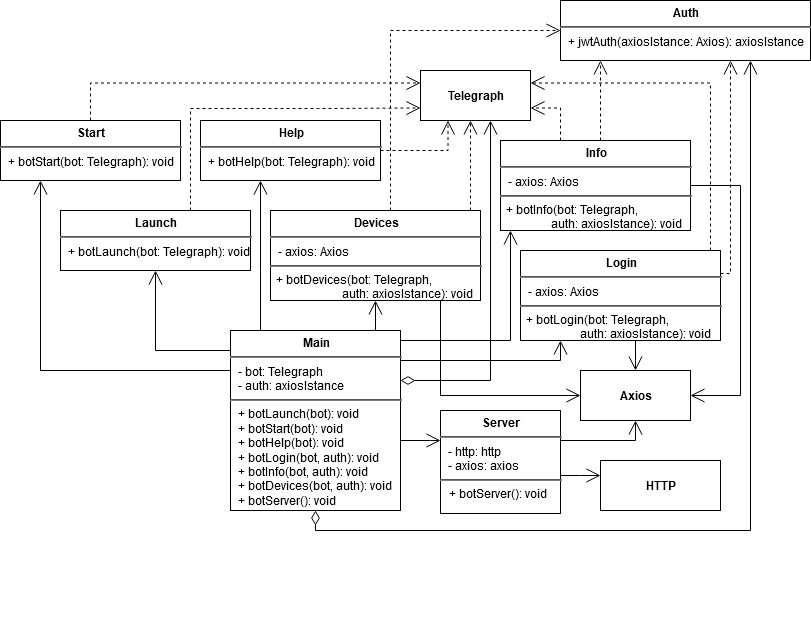
\includegraphics[scale=0.600]{res/images/BOTTELEGRAM/ClassiTelegram.png}
		\caption{Diagramma delle classi della componente bot Telegram}
		\label{Diagramma 19}
	\end{figure}
	Nel diagramma in figura sono presenti le seguenti parti:
	\begin{itemize}
		\item \textbf{Main}: questa parte racchiude tutte le richieste ed i comandi che è possibile effettuare dal bot e per questo ha delle dipendenze verso tutti i comandi disponibili, oltre che verso il modulo Telegraf;
		\item \textbf{Server}: questa componente viene utilizzata per implementare le funzionalità di ricezione di richieste da parte delle API per quanto riguarda l'invio di alert o l'invio del 2FA token. Ha un riferimento verso HTTP e Axios;
		\item \textbf{Start}: questa componente è necessaria per permettere ad un utente di far partire un'istanza del bot Telegram sul proprio dispositivo;
		\item \textbf{Help}: il compito il questa componente è implementare il comando "help" e mostrare di conseguenza la lista di tutti i comandi disponibili agli utenti oltre che una breve descrizione della procedura di autenticazione tramite Telegram;
		\item \textbf{Devices}:il compito di questa componente è implementare il comando "devices": questo comando mostra agli amministratori una lista di tutti i dispositivi che possiedono almeno un sensore abilitato alla ricezione dei comandi. In seguito è possibile selezionare un dispositivo, un sensore ed infine scegliere quale comando inviare. Ha dei riferimenti verso Axios e Telegraf/Markup;
		\item \textbf{Info}: il compito di questa componente è implementare il comando "info", permettendo di visualizzare le informazioni del proprio account. Ha un riferimento verso Axios; 
		\item \textbf{Login}: il compito di questa componente è implementare il comando "login", permettendo all'utente di autenticarsi ed autorizzare il proprio account Telegram all'esecuzione dei diversi comandi. Ha un riferimento verso Axios; 
		\item \textbf{Config}: questa componente ha li compito di caricare i comandi disponibili del proprio bot in modo da abilitare la funzione di suggerimento dei comandi all'interno del bot Telegram. Ha un riferimento verso Axios;
		\item \textbf{jwtAuth}: questa componente è utilizzata per implementare una parte del comando "login". Più in dettaglio imposta il token di autenticazione ottenuto tramite le API.
	\end{itemize}
\subsubsection{Dipendenze esterne}	
	La componente ha tre dipendenze esterne:
	\begin{itemize}
		\item \textbf{Telegraf}, modulo che permette di collegarsi con le API ufficiali di \glock{Telegram}. Ogni comando ne ha un riferimento;
		\item \textbf{Axios}, modulo che permette di effettuare richieste POST e GET e di ritornare una risposta. Viene utilizzato da Server, Login e Status per comunicare con le API e per inviare uno o più messaggi agli utilizzatori del bot;
		\item \textbf{HTTP}, modulo che permette di creare un server HTTP per restare in ascolto di eventuali richieste. Viene utilizzato da Server per ascoltare eventuali richieste delle API.    
	\end{itemize}
\subsubsection{Diagramma di sequenza}%%%%%%%%%OK
	\begin{figure}[H]
		\centering
		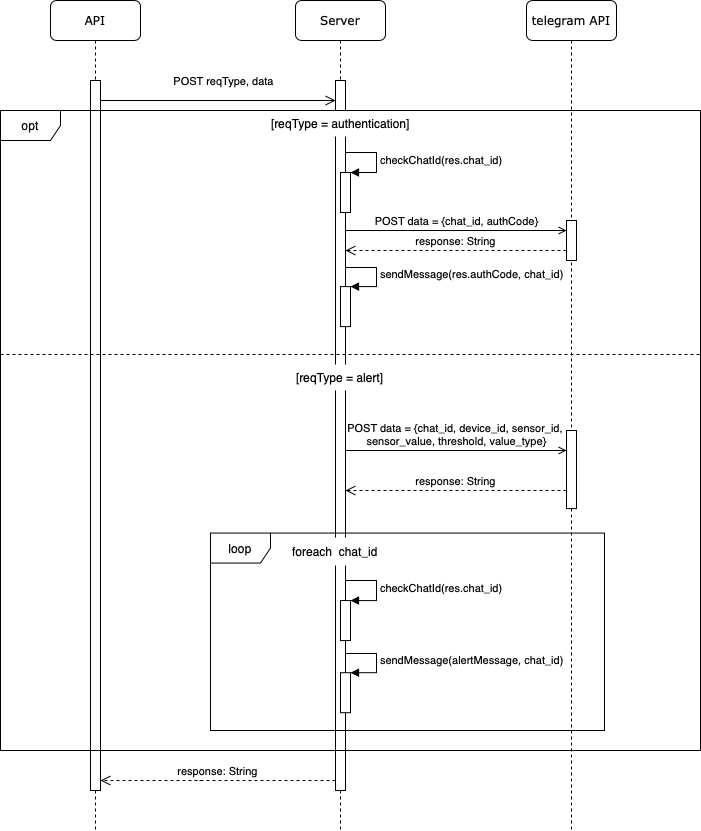
\includegraphics[scale=0.500]{res/images/BOTTELEGRAM/TelegramRichiestaPOST.png}
		\caption{Diagramma di sequenza che riporta la ricezione di una richiesta POST delle API all'interno della componente bot Telegram}
		\label{Diagramma 20}
	\end{figure}

	Nel diagramma di sequenza in alto viene mostrata la ricezione di una richiesta POST dalle API. La richiesta può essere di due tipologie: 
	\begin{itemize}
		\item \textbf{authentication:} in cui vengono inviati dalle API un chat Id ed un codice di autenticazione; quest'ultimo dovrà poi essere inviato al chat Id specificato per permettere all'utente l'autenticazione sulla \glock{web app};
		\item \textbf{alert:} in cui vengono mandati dalle API una lista di chat id ed un insieme di dati che poi andranno composti in un messaggio ed inviati a tutti i chat Id specificati.
	\end{itemize}
\subsubsection{Estensione}
	\paragraph{Inserimento di un nuovo comando}
		Per inserire un nuovo comando all'interno del bot è necessario creare un file .js all'interno della cartella commands.
		\newline
		Poiché sarà poi necessario esportare questo comando, per poi inserirlo all'interno di main.js, l'intestazione del nuovo comando dovrà essere del tipo:
		\begin{verbatim}const botNomeComando = (bot) => {
								bot.command( "nomeComando", (param) => {
							 		...
							 	});
						}; 
		\end{verbatim}	